\documentclass[10pt,a4paper]{amsart}
\usepackage[margin=19mm]{geometry}
\usepackage{amsmath,amssymb,mathtools}
\usepackage[scr=rsfs,cal=euler]{mathalfa}
\usepackage{xfrac}
\usepackage[unicode,hidelinks,bookmarks=false]{hyperref}
\newcommand{\ie}{i.e.\ }
\newcommand{\cf}{cf.\ }
\newcommand{\resp}{respectively\ }
\newcommand{\Subsection}{\subsection}
\providecommand{\nobreakdash}{\nobreak\hbox{-}}
\setlength{\emergencystretch}{2em}
\multlinegap0pt
\usepackage{tikz}
\usepackage{mathtools}
\usepackage{amssymb}
\usepackage{dsfont}
\usepackage{enumerate}
\newtheorem{definition}{Definition}
\newtheorem{lemma}{Lemma}
\newtheorem{proposition}{Proposition}
\newcommand{\R}{\mathbb{R}}
\newcommand{\dist}{\mathrm{dist}}
\title{Sharp bottom spectrum and scalar curvature rigidity}
\author{Jinmin Wang, Bo Zhu}
\date{Source: arXiv:2408.08245v4 (CC BY 4.0)}
\begin{document}
\maketitle

\noindent\emph{Source and licence.} Sharp bottom spectrum and scalar curvature rigidity. Version arXiv:2408.08245v4 (CC BY 4.0), distributed by arXiv under the Creative Commons Attribution 4.0 International licence, http://creativecommons.org/licenses/by/4.0/, as recorded in the arXiv licence metadata for this exact version and shown on the abstract page https://arxiv.org/abs/2408.08245v4. Full licence notice: \texttt{licenses/arxiv-2408.08245-CC-BY-4.0.txt}.\par\smallskip

\noindent\textit{Editorial scope.} Counted unit: the article's proposition prop:interpolation (source0.tex lines 1330--1337). The article's complete original proof of it is delivered with it (source0.tex lines 1338--1410, one \texttt{proof} environment of 73 lines). No mathematics is written, repaired or re-derived: the statement and the proof are the article's own lines, in the article's own notation, and no retained line is substituted or re-flowed.  Retained uncounted as the source-local context the proof needs: lines 918--920; lines 1186--1198; lines 1188--1190; lines 1205--1210; lines 1240--1246; lines 1265--1270.  Nothing was omitted from any retained span, so the package carries no omission record.  No retained line contains a citation, so the wrapper carries no bibliography and no bibliography entry.  The retained lines contain the article's own diagram code, which the wrapper typesets with the standard tikz packages; no image file is delivered and the package declares no asset dependency.  Editorial formatting only, in addition: an AMS \texttt{amsart} preamble that restates the article's own declarations and macros used by the retained lines, namely the environments \texttt{definition}, \texttt{lemma}, \texttt{proposition} on separate counters, together with the standard packages those lines need.  The retained environments print in this document as Definition 1, Lemma 1, Proposition 1 in order of appearance, whereas the article prints the same items with the numbering of its own full document.  The complete native source of the article as distributed in the arXiv e-print for this exact version is bundled unchanged as \texttt{sources/163828/source0.tex}.
\begin{definition}\label{def:net}
	Suppose that  $(X, d)$ is a metric space and $S$ is a subset of $X$. $S$ is said to be  a \emph{net} of $X$ if there exists $r>0$ such that $N_r(S)=X$, where $N_r(S) = \{x \in X: \dist(x, S) < r\}$. Furthermore, we say that $S$ is a \emph{discrete net} of $X$ if there exists $r'>0$ such that $d(x,y)\geq r'$ for any $x\ne y$ in $S$.
\end{definition}

\begin{lemma}\label{lemma:localZ}
	There exists $C_1>0$ such that for any $g\in\mathcal F_Z$, we have
	\begin{equation} \label{eq:localZ}
		\int_{X\times\R_{\geq 0}}\Big(\frac 1 h|\frac{\partial g}{\partial t}g|^2+\frac 1 h|\nabla g|^2+\frac{1}{h^3}|g|^2 \Big)e^{2\varphi_Z/h} \leq C_1\int_{X\times\R_{\geq 0}}e^{2\varphi_Z/h}|Qg|^2
	\end{equation}
%	\begin{equation}
	%	\begin{split}
	%		&\int_{X\times\R_{\geq 0}}e^{2\varphi_Z/h}|Qg|^2\\\geq
	%		 &C_5\int_{X\times\R_{\geq 0}}\Big(\frac 1 he^{2\varphi_Z/h}|\frac{\partial}{\partial t} g|^2+\frac 1 he^{2\varphi_Z/h}|\nabla g|^2+\frac{1}{h^3}e^{2\varphi_Z/h}|g|^2\Big)
	%	\end{split}
%	\end{equation}
	for any $h>0$ sufficiently small.
\end{lemma}

	\begin{equation} 
		\int_{X\times\R_{\geq 0}}\Big(\frac 1 h|\frac{\partial g}{\partial t}g|^2+\frac 1 h|\nabla g|^2+\frac{1}{h^3}|g|^2 \Big)e^{2\varphi_Z/h} \leq C_1\int_{X\times\R_{\geq 0}}e^{2\varphi_Z/h}|Qg|^2
	\end{equation}

\begin{lemma}\label{lemma:interpolation}
	Let $\alpha,\beta,\gamma$ be positive numbers with $\alpha\leq A\beta$ for some $A>0$. If there exist $p,q>0$ and $h_0>0$ such that
	$$\alpha\leq e^{-p/h}\beta+e^{q/h}\gamma$$
	for any $h\in(0,h_0)$, then there exist $C>0$ and $\nu\in(0,1)$ that only depends on $A,p,q,h_0$ such that
	$$\alpha\leq C\beta^\nu\gamma^{1-\nu}.$$
\end{lemma}

\begin{lemma}\label{lemma:iteratedInterpolation}
	Suppose that  $\alpha_i>0$ for $i=0,1,\cdots,N$ and $\beta,\gamma$ are positive numbers with $\alpha_i\leq \beta$ for any $i$. If there exists $\nu\in(0,1)$ and $C\geq 1$ such that 
	$$\alpha_{k+1}\leq C\beta^\nu(\alpha_{k}+\gamma)^{1-\nu},\ k = 0, \cdots, N-1$$
	 then,
	$$\alpha_N\leq C'\beta^\mu(\alpha_{0}+\gamma)^{1-\mu},$$
	where $\mu=1-(1-\nu)^N$ and $C'=(2C)^{1+(1-\nu)+\cdots+(1-\nu)^{N-1}}$.
\end{lemma}

\begin{lemma}\label{lemma:interpolation1}
	Suppose that $X$ is a complete Riemannian manifold, and $Y$ is a discrete net in $X$, and $a$ is a small positive number. Given small positive numbers  $\tau \ll t_0<T\ll a$ and $a_1\ll a$, there exists $C>0$ and $\nu\in(0,1)$ such that,  for any smooth section $\sigma$ of $E$ over $X\times\R_{\geq 0}$, we have
		\begin{equation*}
		\|\sigma\|_{H_1(N_{a_1}(Y)\times N_\tau(t_0))}\leq C \|\sigma\|_{H_1(X\times[0,T])}^\nu\Big(\|Q\sigma\|_{L^2(X\times[0,T])}+\Big\|\frac{\partial \sigma}{\partial t}\Big\|_{L^2(N_a(Y)\times\{0\})}\Big)^{1-\nu}.
	\end{equation*}
\end{lemma}

\begin{proposition}\label{prop:interpolation}
		Let $Y$ be a discrete net in $X$ and $a$ a small positive number. Given small positive numbers $\tau\ll t_0<T\ll a$, there exists $C>0$ and $\nu\in(0,1)$ such that for any smooth section $\sigma$ of $E$ over $X\times\R_{\geq 0}$, we have
	\begin{equation}\label{eq:interpolation}
	\begin{split}
			&\|\sigma\|_{H_1(X\times N_\tau(t_0))}\\\leq &C \|\sigma\|_{H_1(X\times[0,T])}^\nu\Big(\|Q\sigma\|_{L^2(X\times[0,T])}+\Big\|\frac{\partial}{\partial t}\sigma\Big\|_{L^2(N_a(Y)\times\{0\})}\Big)^{1-\nu}.
	\end{split}
	\end{equation}
\end{proposition}

\begin{proof}
	We shall prove that there exists $\varepsilon>0$ such that
		\begin{equation}\label{eq:interpolationH1}
		\begin{split}
			&\|\sigma\|_{H_1(N_{a_1+\varepsilon}(Y)\times N_\tau(t_0))}\\\leq &C_1 \|\sigma\|_{H_1(X\times[0,T])}^{\nu_1}\Big(\|Q\sigma\|_{L^2(X\times[0,T])}+\|\sigma\|_{H_1(N_{a_1}(Y)\times N_\tau(t_0))}\Big)^{1-\nu_1}.
		\end{split}
	\end{equation}
	for some $C_1>0$ and $\nu_1>0$. By Definition \ref{def:net}, there are only finitely many steps to exhaust $X$ from $Y$ by increasing $\varepsilon$ of the neighborhood of $Y$. Since $X$ has bounded geometry, Lemma \ref{lemma:interpolation1}, Lemma \ref{lemma:iteratedInterpolation} and line \eqref{eq:interpolationH1} together implies line \eqref{eq:interpolation}.
		\begin{figure}[h]
		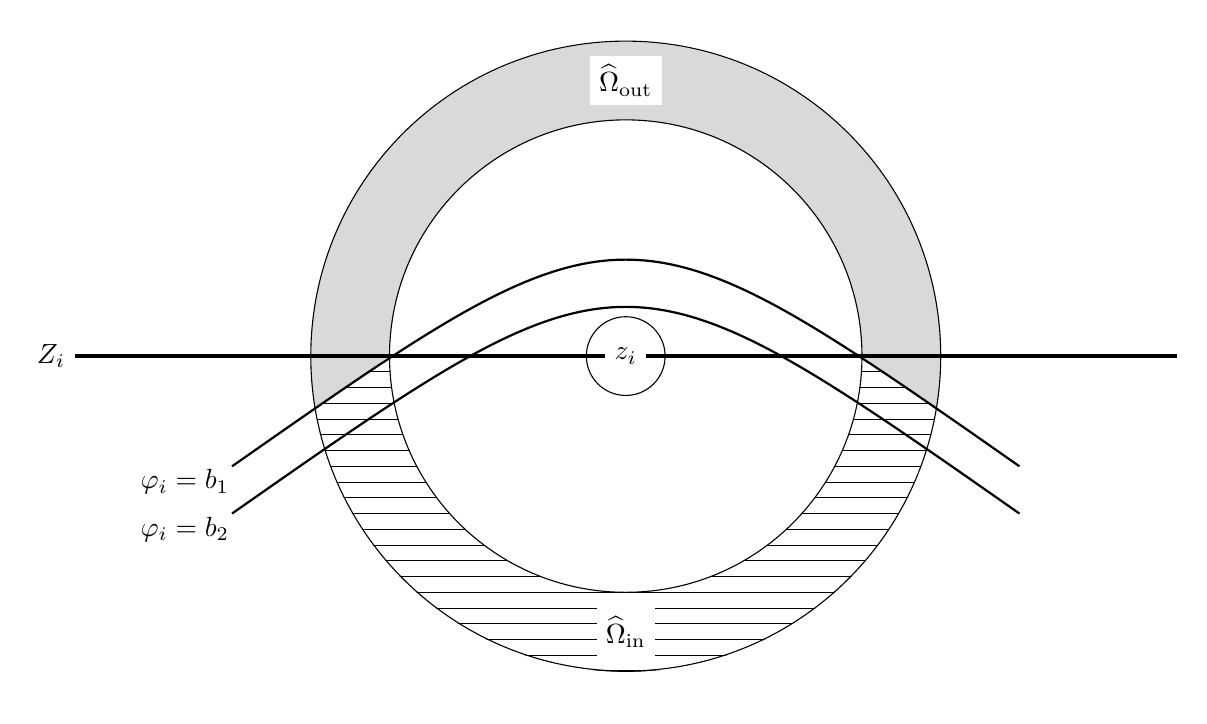
\begin{tikzpicture}[scale=1]\label{fig}
			\node at (-7.3,0){$Z_i$};
			\node at (-5.6,-2.2){$\varphi_i=b_2$};
			\node at (-5.6,-2.2+.6){$\varphi_i=b_1$};
			\fill[gray,opacity=0.3] (3.943,-0.67) arc(-9.5:189.5:4) -- (-3,0) arc (180:0:3) -- cycle;
			\node at (0,3.5)[fill=white]{$\widehat\Omega_{\text{out}}$};
			\draw (0,0) circle[radius=0.5];
			\draw[very thick] (-7,0) -- (7,0);
			\fill (0,0) circle[radius=0.05];
			\draw (0,0) circle[radius=3];
			\draw (0,0) circle[radius=4];
			\draw[thick] (-5,-2) .. controls (0,1.5) .. (5,-2);
			\draw[thick] (-5,-2+.6) .. controls (0,1.5+.6) .. (5,-2+.6);
			\node at (0,0)[fill=white]{$z_i$};
			%\fill (3.943,-0.67) circle[radius=0.05];
			\path[clip] (3.943,-0.67) arc(-9.5:-170.5:4) -- (-3,0) arc (-180:0:3) -- cycle;
			\foreach \y in {0,-.2,...,-4}
			\draw (-4,\y) -- (4,\y);
			\node at (0,-3.5)[fill=white]{$\widehat\Omega_{\text{in}}$};
		\end{tikzpicture}
	\end{figure}
	
	We shall prove line \eqref{eq:interpolationH1} by applying Lemma \ref{lemma:localZ} with carefully chosen $Z$ and $\varphi_Z$. Once chosen, the rest of the proof is completely similar to the proof of Lemma \ref{lemma:interpolation}. 
	Given $N_{a_1}(Y)=\cup_i N_{a_1}(y_i)$, let $z_i$ be a point on $\partial N_{a_1}(y_i)$, $Z_i$ a tiny piece of $\partial N_{a_1}(y_i)$ near $z_i$, and $Z=\cup_iZ_i$. 
	Pick smooth functions $v_i$ supported near $Z_i$ such that $|\nabla v_i|=1$, $Z_i$ is the level set $\{v_i=0\}$, and $\nabla v_i$ is pointing outward from $Z_i\subset \partial N_{a_1}(Y)$. We consider the function $\varphi_Z$ on $X\times\R_{\geq 0}$ such that
	$$\varphi_Z(x,t)=-v_i-d((x,t),(z_i,t_0))^6$$
	near each $Z_i$. 
	
	Let $\chi$ be a smooth cut-off function that is equal to $1$ on $N_{\varepsilon_1}(Z\times\{t_0\})$ and equal to $0$ outside $N_{\varepsilon_2}(Z\times\{t_0\})$. Denote $\widehat\Omega=N_{\varepsilon_2}(Z\times\{t_0\})-N_{\varepsilon_1}(Z\times\{t_0\})$, which contains the supported of $\nabla\chi$.
	Similar to the proof of Lemma \ref{lemma:interpolation}, we define
	$$\Omega_b=\{(x,t)\in N_{\varepsilon_1}(Z\times\{t_0\}):\varphi_Z(x,t)\geq b\}.$$
	By construction of $\varphi_Z$, we have $\varphi_Z(z_i,t_0)=0$, and there exists $b_1<0$ such that $\Omega_{b_1}\cap\widehat\Omega$ is contained inside $N_{a_1}(Y)\times N_\tau(t_0)$. Pick $b_2,b_3$ with $b_1<b_2<0<b_3$ and $\varepsilon>0$ such that $N_\varepsilon(Z)\times N_\tau(t_0)\subset \Omega_{b_2}$ and $N_{\varepsilon_2}(Z\times\{t_0\})\subset (\Omega_{b_3})^c$. 
	
	Now we consider the section $\chi\sigma$, which lies in $\mathcal F_Z$ by assumption, hence satisfies the inequality in Lemma \ref{lemma:localZ}. Similar to the computation in the proof of Lemma \ref{lemma:interpolation1}, the right-hand side of line \eqref{eq:localZ} satisfies the following:
	\begin{align*}
	\int_{X\times\R_{\geq 0}}\frac 1 he^{2\varphi_Z/h}\Big(|\frac{\partial}{\partial t} (\chi\sigma)|^2+|\nabla (\chi\sigma)|^2\Big)\geq&\int_{N_\varepsilon(Z)\times N_\tau(t_0)}\frac 1 he^{2\varphi_Z/h}\Big(|\frac{\partial}{\partial t} (\chi\sigma)|^2+|\nabla (\chi\sigma)|^2\Big)\\
	\geq &\frac 1 he^{2b_2/h}\int_{N_\varepsilon(Z)\times N_\tau(t_0)}\Big(|\frac{\partial}{\partial t} (\chi\sigma)|^2+|\nabla (\chi\sigma)|^2\Big),
	\end{align*}
	and
	\begin{align*}
		\int_{X\times\R_{\geq 0}}\frac{1}{h^3}e^{2\varphi_Z/h}|\chi\sigma|^2\geq \frac{1}{h^3}e^{2b_2/h}\int_{N_\varepsilon(Z)\times N_\tau(t_0)}|\sigma|^2.
	\end{align*}	
	For the left-hand side of line \eqref{eq:localZ}, we still notice that 
	$$Q(\chi\sigma)=\chi Q\sigma+[Q,\chi]\sigma,$$
	where $[Q,\chi]$ is a first-order differential operator that is supported only on $\widehat\Omega$. Write $\widehat\Omega=\widehat\Omega_{\text{in}}\cup \widehat\Omega_{\text{out}}$, where $\widehat\Omega_{\text{in}}\coloneqq \Omega_{b_1}\cap\widehat\Omega$ and $\widehat\Omega_{\text{out}}$ is the complement of $\widehat\Omega_{\text{in}}$. We note that by construction, $\widehat\Omega_{\text{in}}$ is contained in $N_{a_1}(Y)\times N_\tau(t_0)$, while on  $\widehat\Omega_{\text{out}}$ we have $\varphi_Z\leq b_1$. Therefore, there exists $c_1>0$ such that
	\begin{align*}
		&\int_{X\times\R_{\geq 0}}e^{2\varphi_Z/h}|Qg|^2\leq \frac 1 2\int_{N_{\varepsilon_1}(Z\times\{t_0\})}e^{2\varphi_Z/h}|\chi Q\sigma|^2+\int_{\widehat\Omega}e^{2\varphi_Z/h}|[Q,\chi]\sigma|^2\\
	\leq &\frac1 2e^{2b_3/h}\int_{L^2(N_{\varepsilon_1}(Z\times\{t_0\}))}|Q\sigma|^2+\int_{\widehat\Omega_{\text{in}}}e^{2\varphi_Z/h}|[Q,\chi]\sigma|^2+\int_{\widehat\Omega_{\text{out}}}e^{2\varphi_Z/h}|[Q,\chi]\sigma|^2\\
	\leq &\frac1 2e^{2b_3/h}\|Q\sigma\|^2_{L^2(X\times[0,T])}+c_1e^{2b_3/h}\|\sigma\|^2_{H_1(N_{a_1}(Y)\times N_\tau(t_0))}+c_1e^{2b_1/h}\|\sigma\|^2_{H^1(X\times[0,T])}
	\end{align*}
	Therefore, by Lemma \ref{lemma:localZ}, there is $c_2>0$ such that
	\begin{align*}
		&e^{2b_2/h}\|\sigma\|_{H^1(N_\varepsilon(Z)\times N_\tau(t_0))}^2\\ \leq& c_2\Big(e^{2b_3/h}\|Q\sigma\|^2_{L^2(X\times[0,T])}+e^{2b_3/h}\|\sigma\|^2_{H_1(N_{a_1}(Y)\times N_\tau(t_0))}+e^{2b_1/h}\|\sigma\|^2_{H^1(X\times[0,T])}\Big).
	\end{align*}
	Equivalently,
	\begin{align*}
		&\|\sigma\|_{H^1(N_\varepsilon(Z)\times N_\tau(t_0))}^2\\ \leq& c_2e^{2(b_1-b_2)/h}\|\sigma\|^2_{H^1(X\times[0,T])}+c_2e^{2(b_3-b_2)/h}\Big(\|Q\sigma\|^2_{L^2(X\times[0,T])}+\|\sigma\|^2_{H_1(N_{a_1}(Y)\times N_\tau(t_0))}\Big).
	\end{align*}
	We note that $b_1-b_2<0$ and $b_3-b_2>0$. It follows together with Lemma \ref{lemma:interpolation} that
	\begin{align*}
		\|\sigma\|_{H^1(N_\varepsilon(Z)\times N_\tau(t_0))}\leq c_3\|\sigma\|^{\nu_1}_{H^1(X\times[0,T])}\Big(\|Q\sigma\|^2_{L^2(X\times[0,T])}+\|\sigma\|^2_{H_1(N_{a_1}(Y)\times N_\tau(t_0))}\Big)^{1-\nu_1}.
	\end{align*}
	for some $c_3>0$ and $\nu_1>0$. Note that as $X$ has bounded geometry $N_{a_1+\varepsilon}(Y)$ is covered by at most $N$ sets, which are of the form $N_\varepsilon(Z)$ for some $Z\subset\partial N_{a_1}(Y)$. This finishes the proof of line \eqref{eq:interpolationH1} with $C_3=Nc_1$, hence completes the proof of line \eqref{eq:interpolation} by the discussion at the beginning.	
\end{proof}

\end{document}
